\chapter{Conceitos básicos do MT}
\label{CapMT}
\section{O Método}

O MT é um método eletromagnético de exploração  que consiste em obter informações de resistividade elétrica de um meio utilizando como sinal flutuações dos campos elétricos e magnéticos induzidos por fontes naturais.

\subsection{Fontes do sinal MT}

As fontes dos campos eletromagnéticos induzidos na terra são oriundas de fenômenos naturais que ocorrem em um largo espectro de frequência ($f$), podemos dividi-las em duas classes de sinais:
\paragraph{Sinais de alta frequência $f>1 Hz$:}

São devidos a fenômenos elétricos que ocorrem entre a atmosfera e ionosfera, principalmente tempestade elétricas (descargas elétricas na superfície da terra) e são conhecidos como \textit{sferics}

\paragraph{Sinais de baixa frequência $f<1 Hz$:}

 São gerados pela interação do vento solar com a magnetosfera e a ionosfera da terra.
  
 A frequência da fonte natural é um dos fatores que controlam a profundidade de alcance da onda eletromagnética e portanto, a profundidade que o método consegue investigar. A profundidade de investigação pode ser determinada pelo \textit{skin depth}, que terá seu conceito melhor abordado mais a frente. A Figura \ref{exploracao} mostra a relação entre a frequência da fonte e a profundidade de investigação com os diferentes tipos de estudos realizados com o MT.  
 
 
 
 %O vento solar é um fluxo contínuo de plasma, irradiando  principalmente prótons e elétrons do Sol e ao encontrar ocampo magnético terrestre, estes prótons e elétrons são desviados em direções opostas, assim estabelecendo um campo elétrico


 
\begin{figure}[!h]
\centering 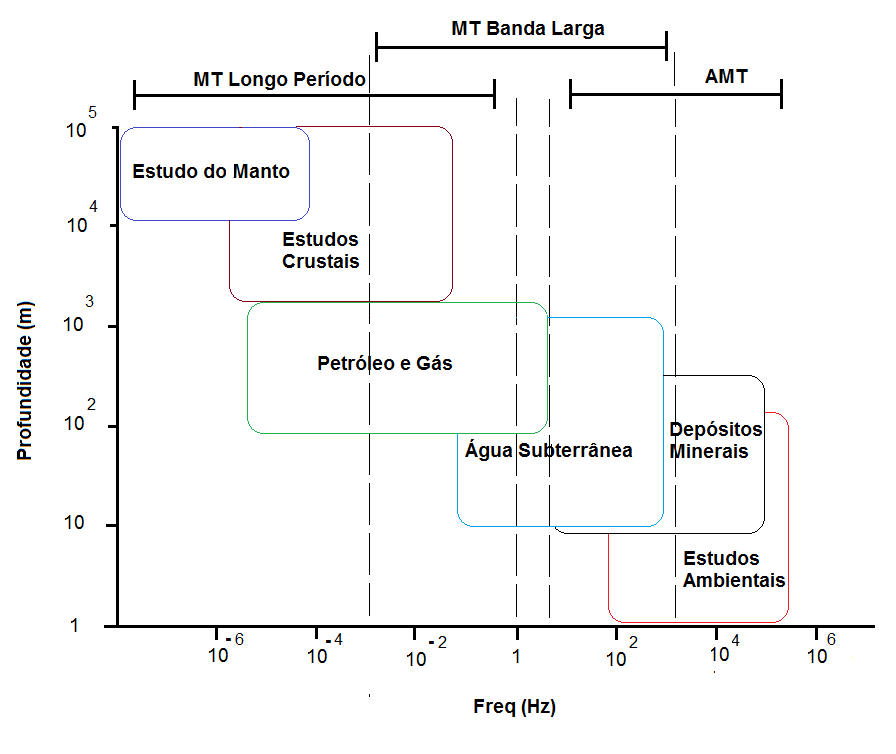
\includegraphics[width=12.5cm,height=10.5cm]{Figs/faixadefrequencias}
\caption{Relação entre as faixas de frequência do sinal e profundidade de investigação com os diversos estudos desenvolvidos com MT.}
\label{exploracao}
\end{figure}


\pagebreak

\section{Teoria do método}
O principio teórico é fundamentado na teoria eletromagnética e nas equações de Maxwell. Afim de se considerar o fenômeno de indução eletromagnética na Terra, são necessárias algumas considerações \cite{simpson2005practical}:

\begin{enumerate}
	\item As equações de Maxwell são obedecidas;
	
	\item Todos os campos gerados são considerados conservativos e analíticos em pontos afastados de suas fontes;
	
	\item  A fonte do campo eletromagnético utilizado no método MT é gerada principalmente por sistemas de correntes localizados na ionosfera, que estão relativamente afastados da superfície da Terra. Esta é tratada como sendo uma onda eletromagnética plano-polarizada, uniforme, que vai de encontro a superfície da Terra verticalmente;
	
	\item Não há acúmulos de cargas livres  em camadas dentro da Terra. Em uma Terra multidimensional as cargas podem ser acumuladas ao longo das continuidades, isto é, a fonte de geração de um fenômeno não indutivo conhecido como \textit{static Shift};
	
	\item A carga é conservativa e se comporta como um condutor ôhmico e obedece a equação $\vec{J}=\sigma\vec{E}$. Onde, $\vec{J}$, $\sigma$ e $\vec{E}$ tem unidade de $Am^{2}$, $Sm^{-1}$ e $Vm^{-1}$, respectivamente; 
	
	\item O deslocamento do campo elétrico é considerado praticamente estático para levantamentos MT. Entretanto, o deslocamento de correntes variantes no tempo (originárias nos efeitos de polarização) são desprezíveis comparadas com as variações das correntes de condução variantes no tempo. Isto promove o tratamento da indução eletromagnética, na Terra, puramente através de processos de difusão;
	
	\item Quaisquer variações nas permissividades elétricas e nas permeabilidades magnéticas existentes nas rochas são consideradas desprezíveis comparadas a variações de condutividades na rocha como um todo.
\end{enumerate} 


\section{Equações de Maxwell e Relações Constitutivas}

A teoria eletromagnética pode ser descrita através das equações de Maxwell na sua forma diferencial e no domínio da frequência:
\begin{itemize}
\item Lei de Faraday
\end{itemize}

\begin{equation}
	\nabla\times\vec{E} = \frac{-\partial \vec{B}}{\partial t}.
\end{equation}

\begin{itemize}
	\item Lei de Ampere
\end{itemize}

\begin{equation}
\nabla\times\vec{H} = \frac{\partial \vec{D}}{\partial t} + \vec{J}.
\end{equation}

\begin{itemize}
	\item Lei de Gauss
\end{itemize}

\begin{equation}
\nabla\cdot\vec{B} = 0.
\end{equation}

\begin{itemize}
	\item Lei de Gauss
\end{itemize}

\begin{equation}
\nabla\cdot\vec{D} = \bar{\rho}.
\end{equation}

 sendo $\vec{E}$ o vetor campo elétrico, $\vec{H}$ ($A/m$) o vetor campo magnético, $\vec{D}$ ($C/m^{2}$) o vetor deslocamento de campo elétrico, $\vec{B}$ ($T$) o vetor indução magnética, $\vec{J}$ o vetor de densidade de corrente elétrica e $\bar{\rho}$ ($C/m^{3}$)a densidade volumétrica de cargas elétricas.
 
As Equações de Maxwell possibilitam o entendimento do comportamento do campo eletromagnético, porém não existe uma relação óbvia entre este comportamento e a estrutura da subsuperfície terrestre e suas propriedades elétricas e magnéticas. Para fazer esta correlação, as equações de Maxwell são complementadas pelas seguintes relações constitutivas \cite{Lugao93}:

\begin{equation}
\vec{D} = \varepsilon \vec{E},
\label{c1}
\end{equation}


\begin{equation}
\vec{B} = \mu \vec{H},
\label{c2}
\end{equation}

\begin{equation}
\vec{J} = {\sigma} \vec{E},
\label{c3}
\end{equation}

Onde $\varepsilon$ $(F/m)$, $\mu$ $(H/m)$ e $\sigma$ são tensores que descrevem, respectivamente, a permissividade elétrica , permeabilidade magnética  e condutividade elétrica do meio, contudo, em um meio isotrópico estas grandezas tornam-se escalares.

As equações \eqref{c1}, \eqref{c2} e \eqref{c3} evidenciam as relações entre os campos elétricos e deslocamento elétrico, magnético e indução magnética e o surgimento de corrente como resposta à presença de campo elétrico externo, respectivamente.

Considerando as relações constitutivas, as equações de Maxwell podem ser expressas em termos de campo elétrico e campo magnético:

\begin{equation}
\nabla\times\vec{E} = -i\mu \omega \vec{H},
\label{max_omega1}
\end{equation}


\begin{equation}
\nabla\times\vec{H} = \sigma\vec{E} + i\omega\varepsilon\vec{E},
\label{max_omega2}
\end{equation}

sendo $\partial/\partial t= i\omega$ e $\omega=2\pi f$.
%\begin{equation}
%\nabla\times\vec{H} = \sigma \vec{E} + \frac{\partial %(\varepsilon\vec{E})}{\partial t}
%\label{max_relacoes1}
%\end{equation}

%\begin{equation}
%\nabla\times\vec{E} = \frac{-\partial (\mu \vec{H})}{\partial t}
%\label{max_relacoes2}
%\end{equation}

%Aplicando o rotacional nas equações acima, considerando que $\vec{E}$ e $\vec{H}$ são contínuos e possuem primeiras e segundas derivadas, obtemos as equações da onda:

Aplicando o rotacional e usando a identidade vetorial $\nabla \times (\nabla \times\vec{A}) = \nabla(\nabla \cdot \vec{A}) - \nabla\cdot\nabla \vec{A}= \nabla(\nabla \cdot \vec{A}) - \nabla^{2}\vec{A}$ ($\vec{A}$ é um vetor arbitrário) nas equações \eqref{max_omega1} e \eqref{max_omega2}, e satisfazendo a condição (6), obtêm-se as equações da difusão dos campos eletromagnéticos:

\begin{equation}
\nabla^{2}\vec{H} = k^{2} \vec{H},
\label{eq_onda_freq1}
\end{equation}

\begin{equation}
\nabla^{2}\vec{E} = k^{2}\vec{E},
\label{eq_onda_freq2}
\end{equation}

%em que $K^{2}= \mu \varepsilon \omega^{2} - i\mu \sigma\omega$. 
em que $k^{2}\cong i\mu \sigma\omega$

Como dito na consideração (2), consideramos uma Terra uniforme, com fontes de sinal homogêneo e localizadas no infinito, de forma que a incidência das
ondas eletromagnéticas sobre a superfície da Terra seja vertical, coincidente com o eixo $z$. Assim , as soluções das equações de difusão para os campos elétricos e magnéticos são da forma:

\begin{equation}
\vec{H}(\omega) = \vec{H}_{0} e^{-i(kz-\omega t)}
\label{eq_sol1}
\end{equation}

\begin{equation}
\vec{E}(\omega) = \vec{E}_{0} e^{-i(kz-\omega t)}
\label{eq_sol2}
\end{equation}


onde $k=\sqrt{-i\omega\mu\sigma}$ é o vetor de onda em módulo que contém informações sobre a direção e o sentido de propagação da onda. $\vec{H}_{0}$ e $\vec{E}_{0}$ são os valores dos campos magnéticos e elétricos na superfície.  


A partir das soluções para equações de difusão dos campos elétricos e magnéticos é possível deduzir uma expressão para a profundidade de investigação. O \textit{skin depth} relaciona a frequência do sinal, a resistividade do meio e a profundidade de penetração da onda eletromagnética, no qual a amplitude da onda decai por um fator de $1/e$. O \textit{skin depth} é matematicamente definido por:

\begin{equation}
	\delta = \sqrt{\frac{2}{\mu_{0}\sigma\omega}},
	\label{skin}
\end{equation}

substituindo $\mu=\mu_{0}=4\pi \times 10^{-7} H/m$ e $\omega=2\pi f$, temos:

\begin{equation}
\delta \approx 503 \sqrt{\frac{\rho}{f}},
\label{skin2}
\end{equation}

onde $\delta$ é dado em metros, $\rho$ $(\Omega/m)$ é a resistividade do meio em que a onda está difundindo e $f$ $(Hz)$ é a frequência. 

Utilizando a convenção geomagnética para coordenadas: $x, y, z$ são positivos em direção ao norte geográfico, ao leste geográfico e ao interior da terra, respectivamente. Uma onda eletromagnética plana caracterizada por $\vec{E}=(E_{x},0,0)$ e $\vec{H}=(0,H_{y},0)$ incide na interface Ar-Terra, Utilizando a equação \eqref{max_omega1} e aplicando as novas condições de polarização acima, têm se:

\begin{equation}
\frac{\partial E}{\partial z} = -ikE_{x}= -i\mu_{0} \omega H_{y},
\label{m1}
\end{equation}

substituindo $k$ na equação acima e reagrupando os termos:
\begin{equation}
\frac{E_{x}}{H_{y}}= (1+i)\sqrt{\frac{\omega\mu_{0}}{2\sigma}},
\label{m2}
\end{equation}

sendo $\rho=1/\sigma$

\begin{equation}
\frac{E_{x}}{H_{y}}= (1+i)\sqrt{\frac{\omega\mu_{0}\rho}{2}},
\label{m3}
\end{equation}

elevando ao quadrado os dois membros da equação acima, obtêm-se:

\begin{equation}
\left[\frac{E_{x}}{H_{y}}\right]^2 =\omega\mu_{0}\rho_{xy},
\label{m4}
\end{equation}

em que $|Z_{xy}|^{2}=\omega\mu_{0}\rho_{xy}$ é uma das componentes do tensor de impedância $Z$ que relaciona $E$ e $H$ em uma direção adotada:

\begin{equation}
E_{x}=Z_{xy}H_{y}
\label{m5}
\end{equation}

A resitividade $\rho_{xy}$ do meio é então:

\begin{equation}
\rho_{xy}= \frac{|Z_{xy}|^{2}}{\omega\mu_{0}}
\label{m6}
\end{equation}

De modo geral, o tensor de impedância pode ser definido como:

	\begin{equation}
	\left[\begin{array}{c}
	E_{x} \\
	E_{y} \\
	\end{array}\right] =
	\left[\begin{array}{cc}
	Z_{xx} &  Z_{xy} \\
	Z_{yx} &  Z_{yy} \\
	\end{array}\right]	\left[\begin{array}{c}
	H_{x} \\
	H_{y} \\
	\end{array}\right]
	\end{equation}
\section{Indução EM 1D}

Um modelo da Terra unidimensional é uma estrutura na qual a condutividade varia apenas com a profundidade ($\sigma = \sigma(z)$).

A resitividade aparente do meio pode ser dada por:
\begin{equation}
	\rho_{a}=\frac{1}{\omega\mu_{0}}\left[\frac{E_{x}}{H_{y}}\right]^2
\end{equation}

Os campos elétricos e magnéticos são ortogonais, as componentes do tensor de impedância tem as seguintes relações com os campos elétricos e magnéticos:

	\begin{equation}
	\left[\begin{array}{c}
	E_{x} \\
	E_{y} \\
	\end{array}\right] =
	\left[\begin{array}{cc}
	0 &  Z_{xy} \\
	-Z_{xy} &  0 \\
	\end{array}\right]	\left[\begin{array}{c}
	H_{x} \\
	H_{y} \\
	\end{array}\right]
	\end{equation}
	
$Z_{yx}=-Z_{xy}$ e $Z_{xx}=Z_{yy}=0$.	
	
\section{Indução EM 2D}

Considerando a indução eletromagnética para um modelo em duas dimensões, o \textit{strike} geoelétrico é paralelo ao eixo $x$, a resistividade varia apenas nas direções $y$ e $z$,  na direção $x$ a resistividade não varia e todas as estruturas estendem ao infinito. Em contraste com o modelo da terra em um dimensão, aqui as componentes $E_{z}$ e $H_{z}$ do campo podem não ser iguais a zero.

Utilizando as equações \eqref{max_omega1} e \eqref{max_omega2}, levando em consideração que $\partial E/ \partial x=0$ e $\partial H/\partial x=0$, podemos separar o conjunto de equações resultantes em modo transverso elétrico (TE) com o conjunto $E_{x}$, $H_{y}$ e $H_{z}$ e modo transverso magnético (TM) com o conjunto $H_{x}$, $E_{y}$ e $E_{z}$.

\begin{description}
	\item [TE] o campo elétrico é polarizado paralelamente a direção de \textit{strike} (eixo $x$), as componentes do campo magnético ficam confinadas no plano (y-z).
\end{description}

\begin{description}
	\item [TM]: o campo magnético está polarizado paralelamente a direção de \textit{strike} geológico, as componentes do campo elétrico ficam confinados no plano (y-z), nesse modo.  
	
\end{description}



\begin{description}
	\item[Tensor de impedância modelo 2D]
	Nesse caso, $Z_{xy}\neq Z_{yx}$
\end{description}

	\begin{equation}
	\left[\begin{array}{c}
	E_{x} \\
	E_{y} \\
	\end{array}\right] =
	\left[\begin{array}{cc}
	0 &  Z_{xy} \\
	Z_{yx} &  0 \\
	\end{array}\right]	\left[\begin{array}{c}
	H_{x} \\
	H_{y} \\
	\end{array}\right]
	\end{equation}

\section{Indução EM 3D}


Considerando a indução em um modelo tridimensional, a resistividade poderá variar nas direções $x$ e $y$ e também com a profundidade, para esse caso o tensor de impedância torna se completo.



	\begin{equation}
	\left[\begin{array}{c}
	E_{x} \\
	E_{y} \\
	\end{array}\right] =
	\left[\begin{array}{cc}
	Z_{xx} &  Z_{xy} \\
	Z_{yx} &  Z{yy} \\
	\end{array}\right]	\left[\begin{array}{c}
	H_{x} \\
	H_{y} \\
	\end{array}\right]
	\end{equation}


%\begin{figure}[hbt]
	
%\centering \subfigure[Condição de contorno não reflexiva
%(CCNR).]{\label{fig:cc_nr}
%\includegraphics[width=6.5cm,height=6.5cm]
%{Figs/cc_nr}} \qquad \subfigure[Camadas de amortecimento +
%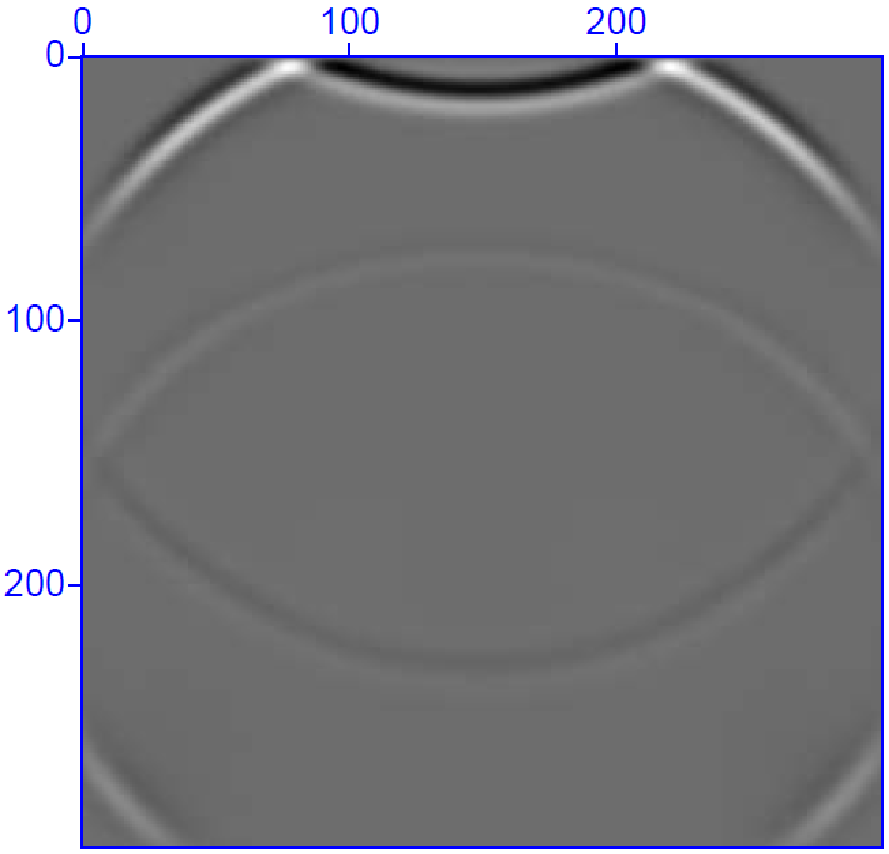
\includegraphics[width=6.5cm,height=6.5cm]{Figs/cerjan}}
%\caption[Exemplo de múltiplas figuras (texto do índice).]{Exemplo de múltiplas
%figuras: modelagem
%acústica mostrando efeito da aplicação da CCNR e camadas de amortecimento
%aplicadas nas bordas (menos na superfície). Aplica-se em (a) as CCNR de
%Reynolds e em (b) as camadas de amortecimento mais CCNR de Reynolds.}
%\label{fig:cc}
%\end{figure}

%Repare para que o exemplo acima funcione corretamente, é necessário a utilização do pacote``\verb|\usepackage{subfigure}|'', declarado no preambulo do documento principal. Para tal, este pacete deve estar instalado no LaTex utilizado para processar o documento. Indicamos a utilização do MikTex (gratuito) mais atual com editor WinEdt (pago).